\documentclass[12pt]{article}
 
\usepackage[margin=1in]{geometry}
\usepackage[font=small,labelfont=bf]{caption}
\usepackage{graphicx}
%\usepackage[draft]{graphicx}
\usepackage{amsmath, amsthm, amssymb, bm, enumitem, nicefrac, float, booktabs, adjustbox, subcaption, fancyhdr, makecell, titlesec, dsfont, epigraph}
\PassOptionsToPackage{hyphens}{url}\usepackage{hyperref}

\newcommand{\N}{\mathbb{N}}
\newcommand{\Z}{\mathbb{Z}}
\DeclareMathOperator*{\argmax}{argmax}
%\DeclareMathOperator*{\argmin}{argmin}
\newcommand{\argmin}{\mathop{\mathrm{argmin}}} 
\setcounter{MaxMatrixCols}{20}


\pagestyle{fancy}
\fancyhead{}
\setlength{\headheight}{15pt}
\setlength{\emergencystretch}{2pt} 
\fancyfoot{}
\fancyhead[L]{\slshape{Treasury Yield Curve}}
\fancyhead[R]{\slshape J.R. Becker}
\fancyfoot[C]{\thepage}


\begin{document}
	
The methodology used for building yield curves follows \cite{termstrc} with a few additions. First, all currently traded treasuries are collected. Following, bonds which have remaining maturities less than the original maturity of another tenor are removed (e.g., 30 year bonds are removed once their maturity is below 10 years, 10 and 7, 7 and 5, etc.). Once these bonds have been removed, the Nelson-Siegel-Svensson method from \cite{termstrc} is used, with the error between inverse-duration weighted prices minimized to efficiently solve for the yield curve (minimizing inverse duration weighted price errors is orders of magnitude faster than yield errors). Bounds on the $\beta$ and $\tau$ parameters are taken from \cite{calibrating}. Randomized grid-search initiations are used to improve the robustness of curves, where random sets of parameters within the given bounds are used as starting points for the optimizer, increasing the probability that at least one finds the global minimum, as the problem is not well-posed. The resulting yield curve at this point is shown in Figure \ref{no_thresh}.\bigskip

In order to smooth the curve and make it more robust, an iterative thresholding process is subsequently performed to remove outliers. The residual between market value and theoretical YTM for each bond is calculated, and bonds with residuals greater than 12 bp are removed from the process. This is repeated until no bonds are removed. Figure \ref{thresh} displays the robust curve generated after this iterative process using the default parameters, where 10 random initiations are used for dropping bonds, and 25 random initiations are used for the final curve after all outliers have been dropped.

\begin{figure}[H]
	\centering
	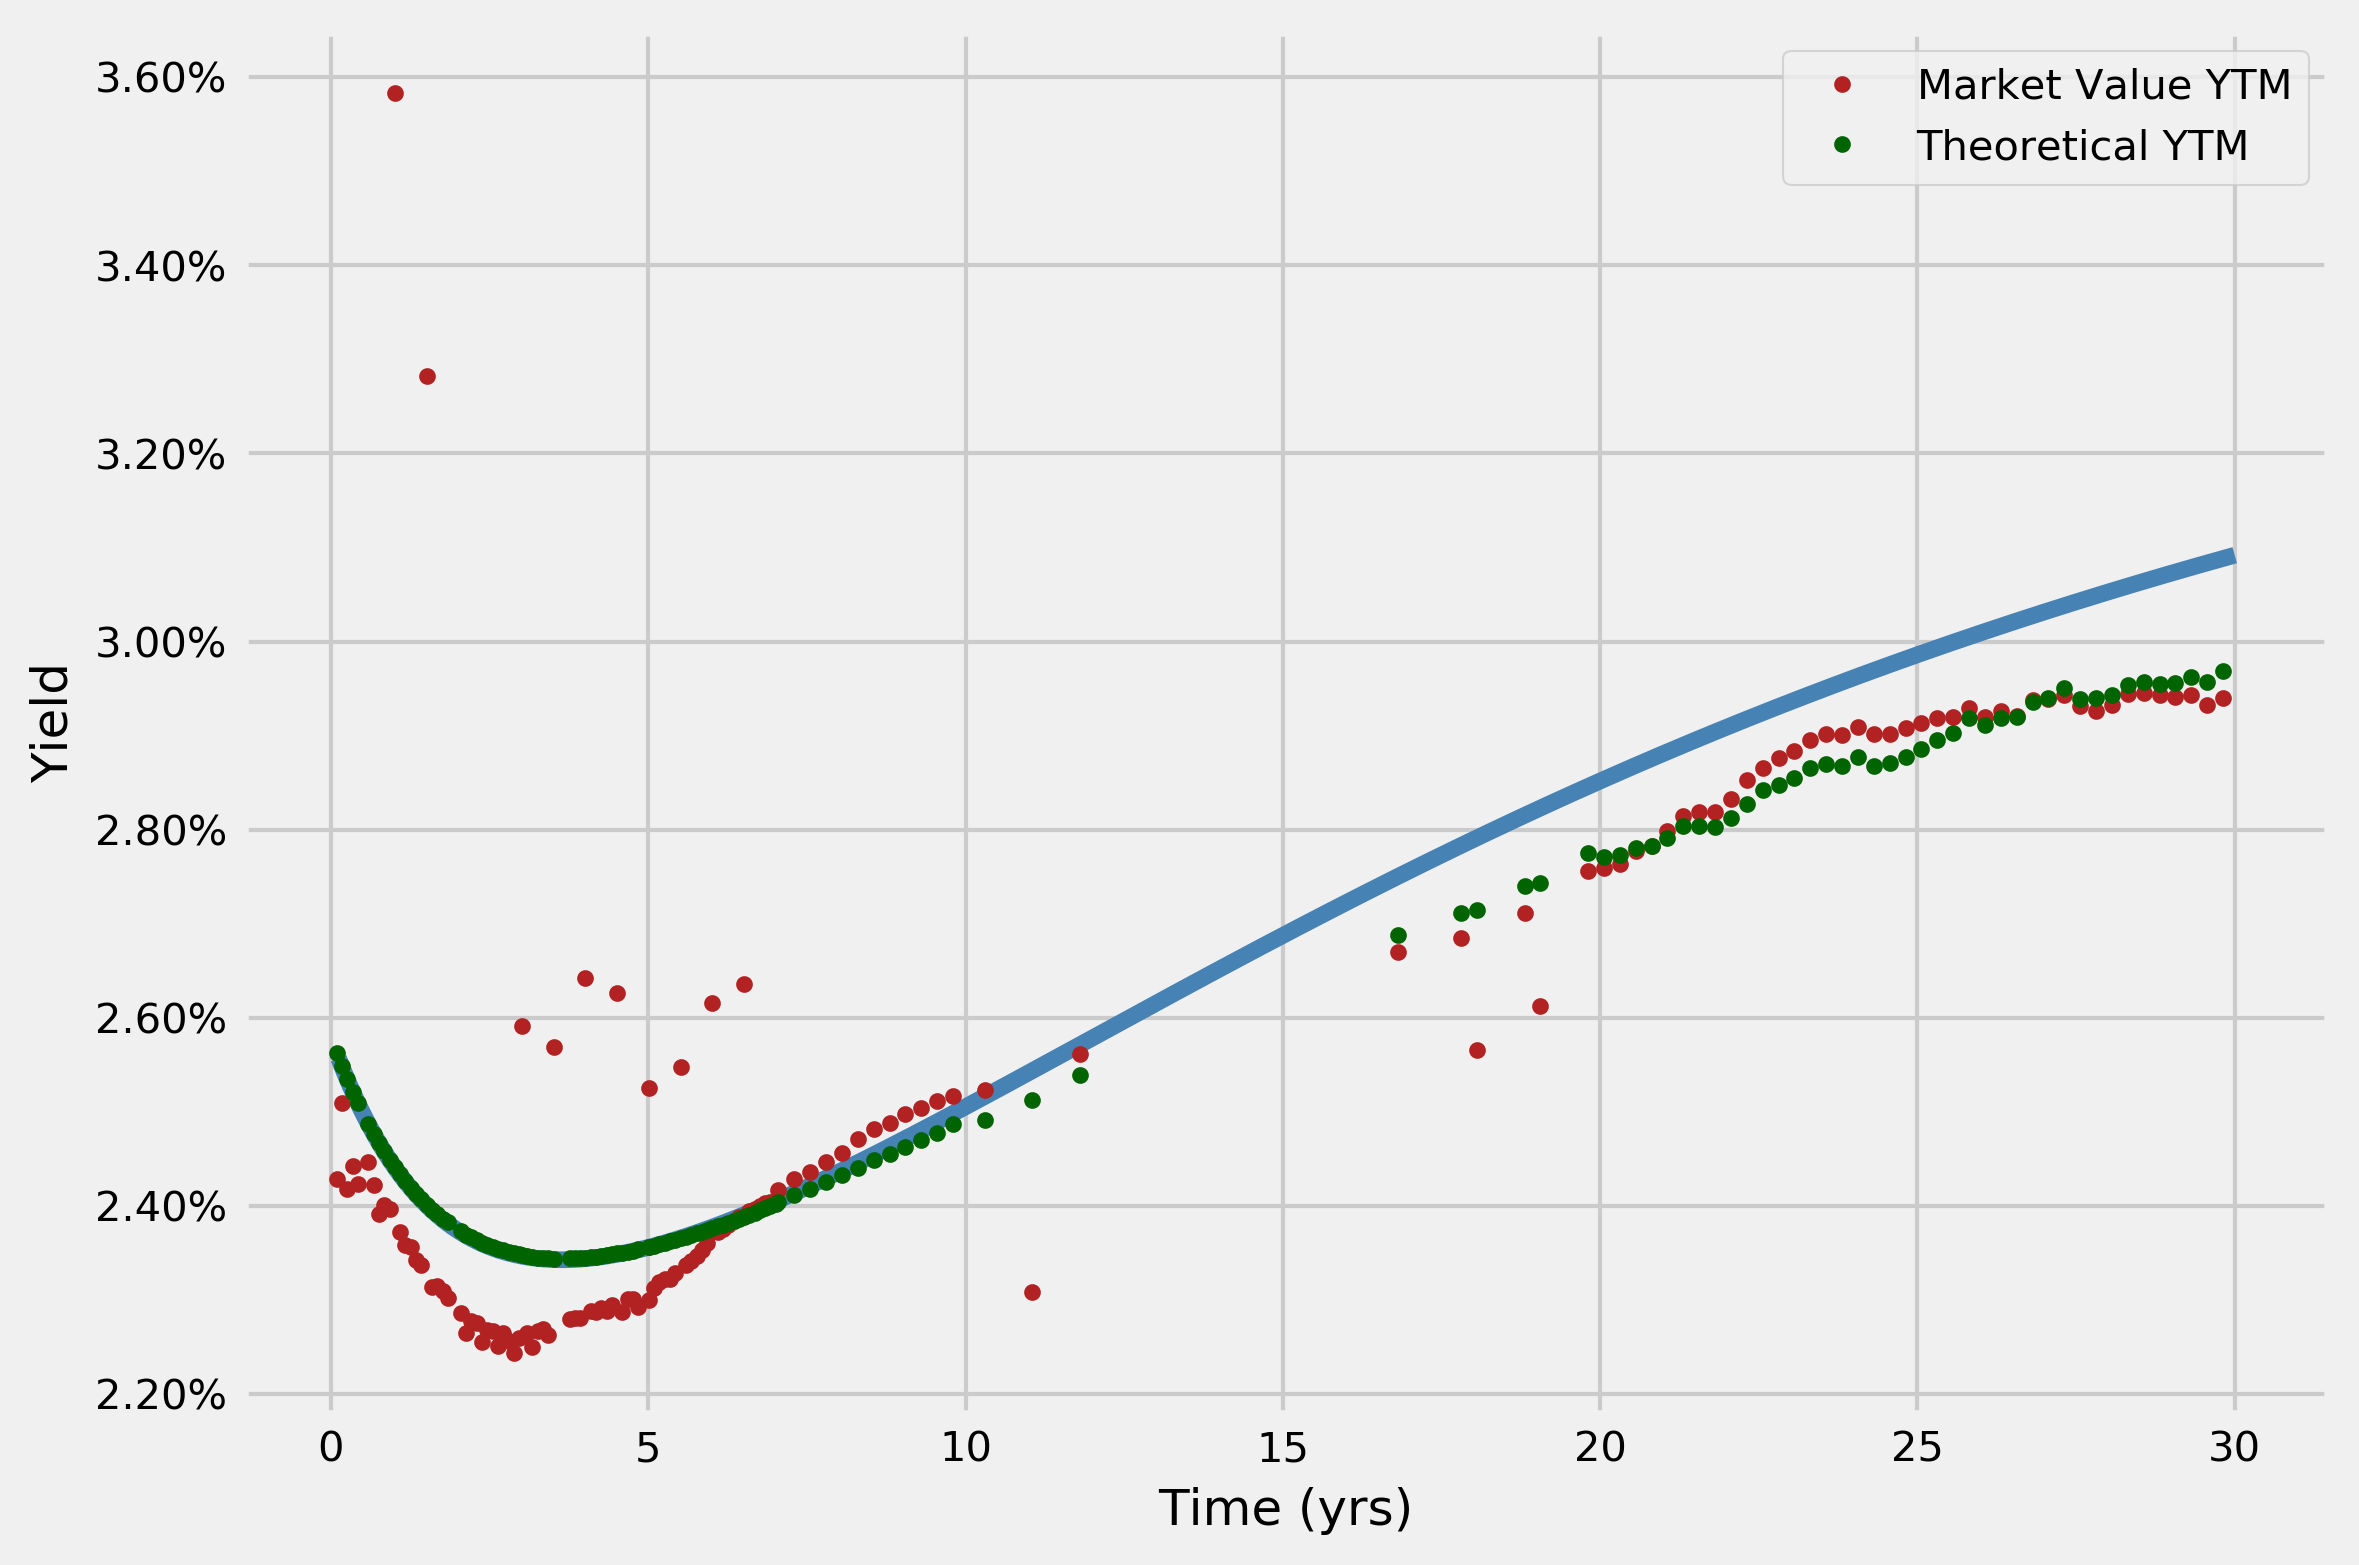
\includegraphics[width=0.9\textwidth]{../../fig/treasury_curves/ytm_no_threshold}
	\caption{Zero curve plotted with all coupon treasuries.}
	\label{no_thresh}
\end{figure}

\begin{figure}[H]
	\centering
	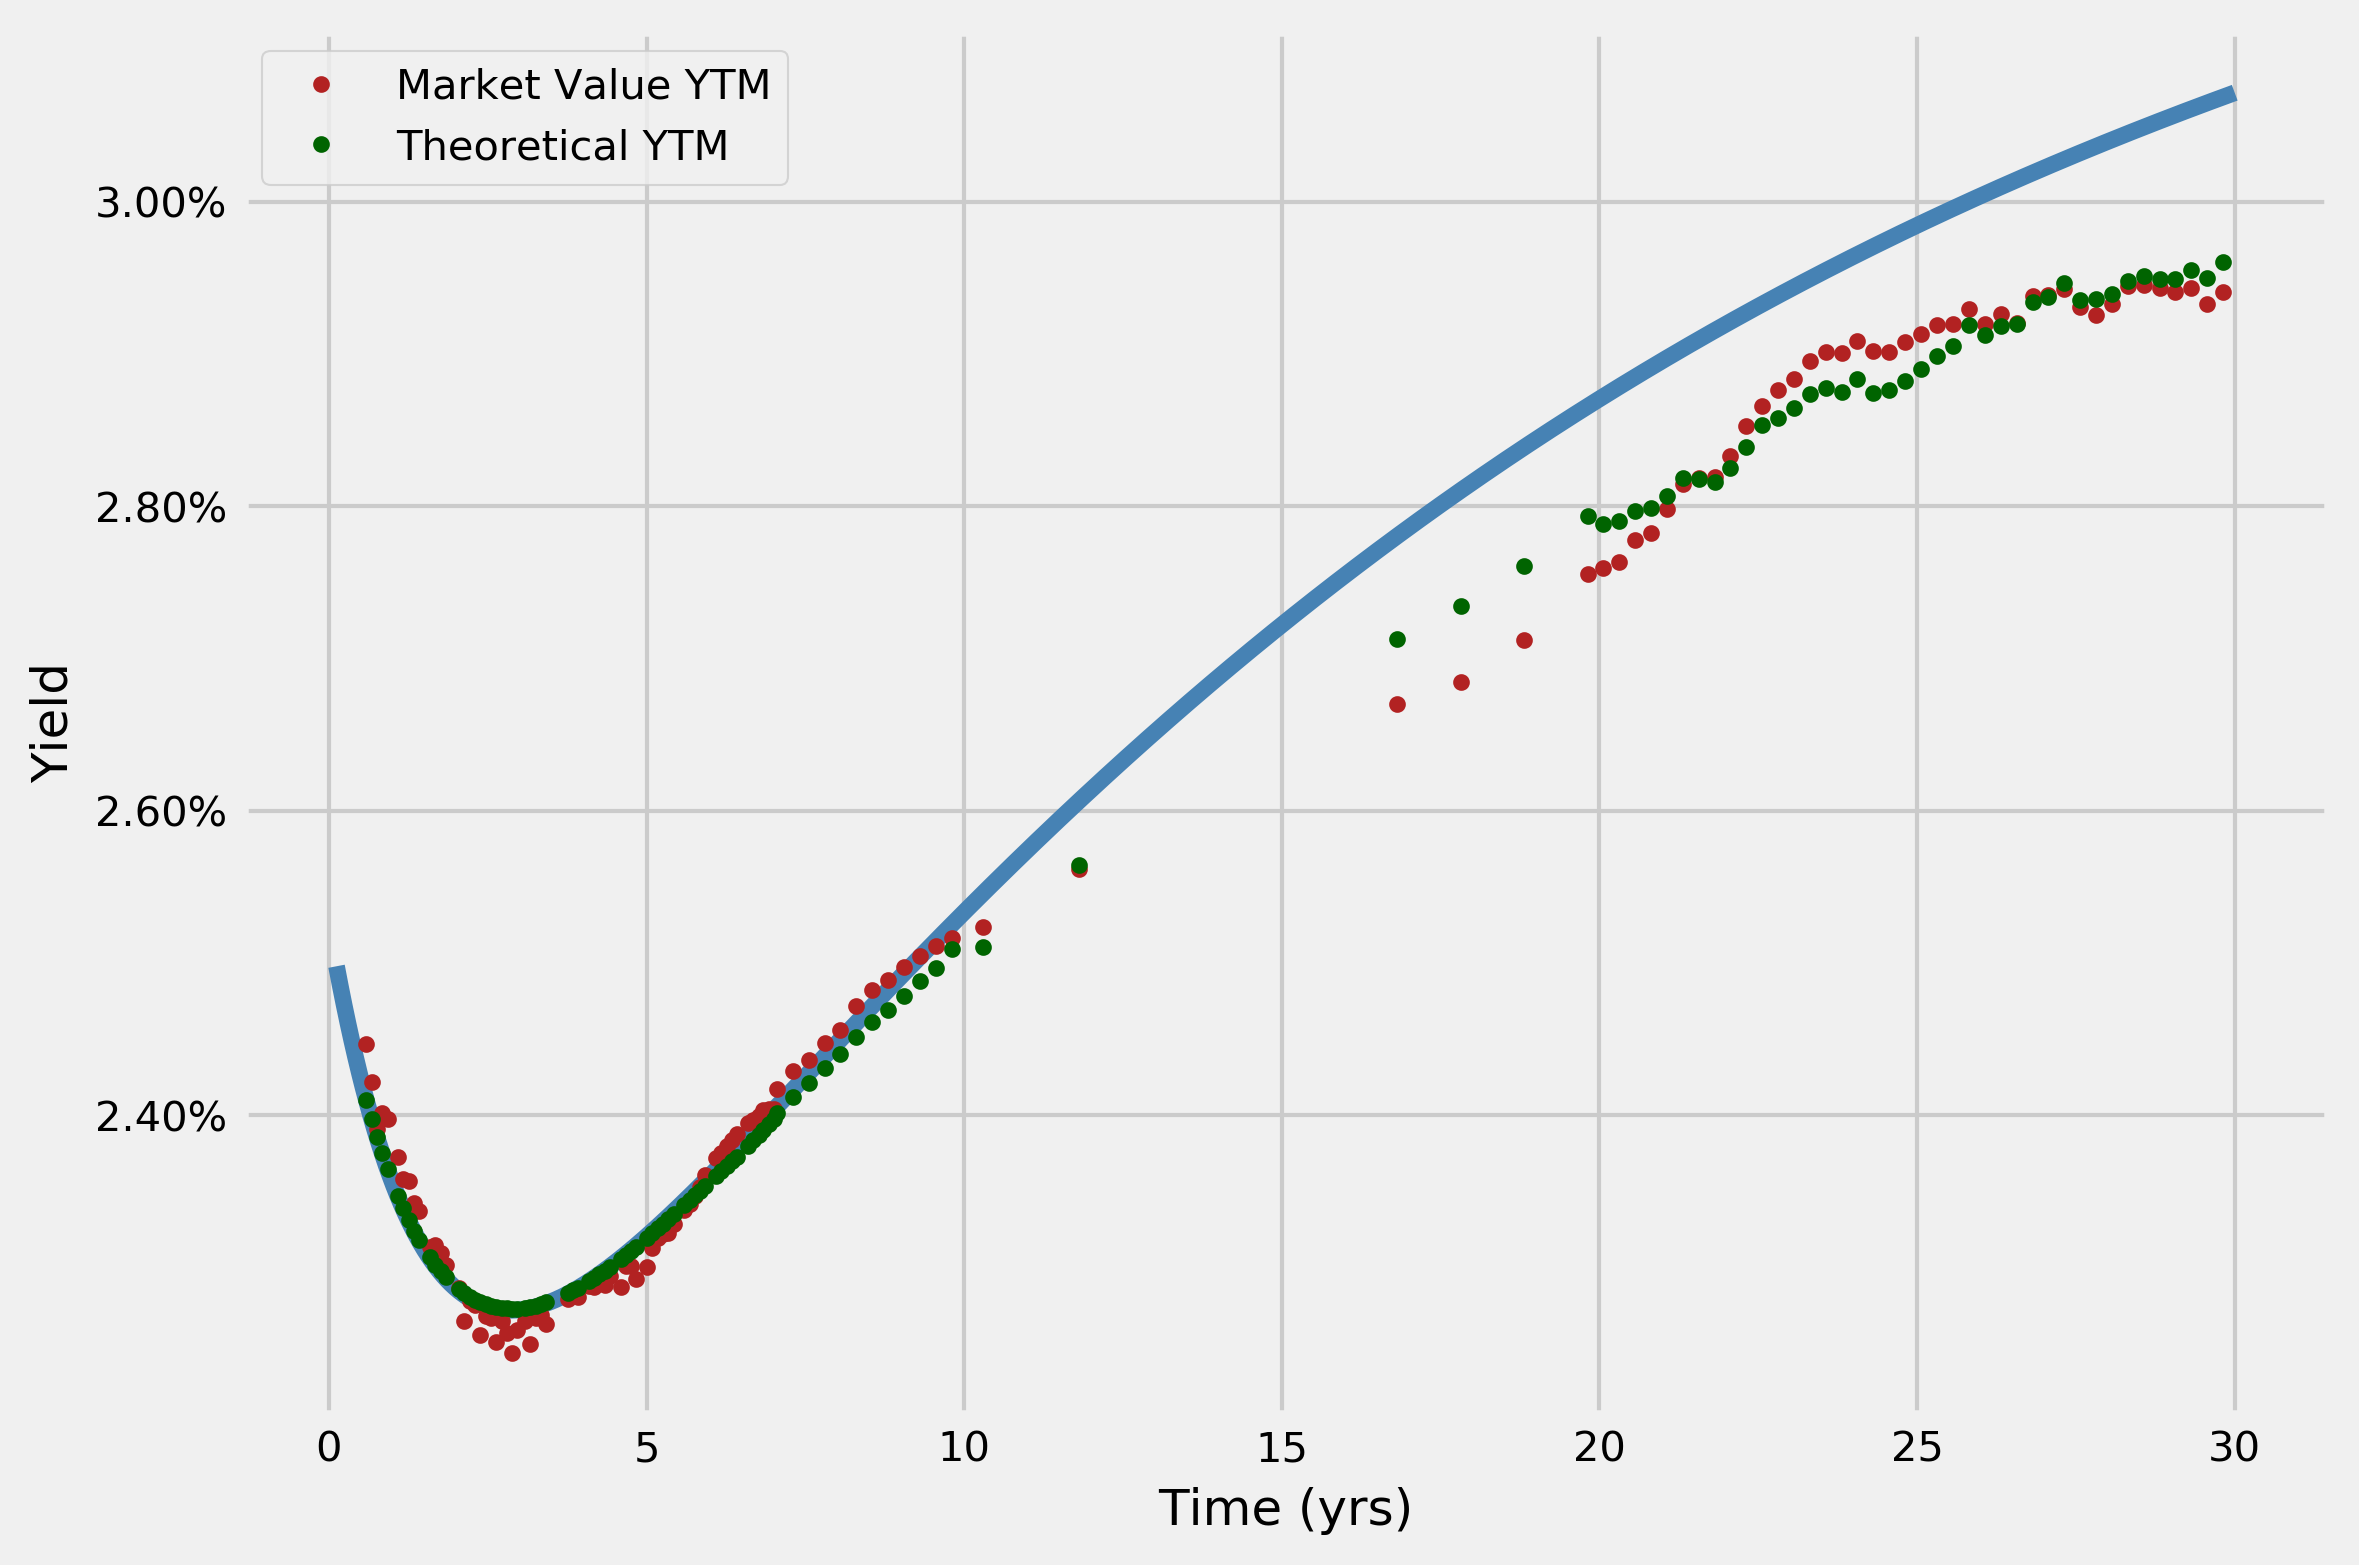
\includegraphics[width=0.9\textwidth]{../../fig/treasury_curves/ytm_threshold}
	\caption{Zero curve after thresholding treasuries. }
	\label{thresh}
\end{figure}


As Figures \ref{no_thresh} and \ref{thresh} contain coupon bonds, the zero curve is higher than the calculated yield to maturities in the back end, making it difficult to test validity. Hence, treasury strips (which are not used in the process of building the curve) are plotted over the final zero curve below for validation that the back of the curve is in line with market zero prices.

\begin{figure}[H]
	\centering
	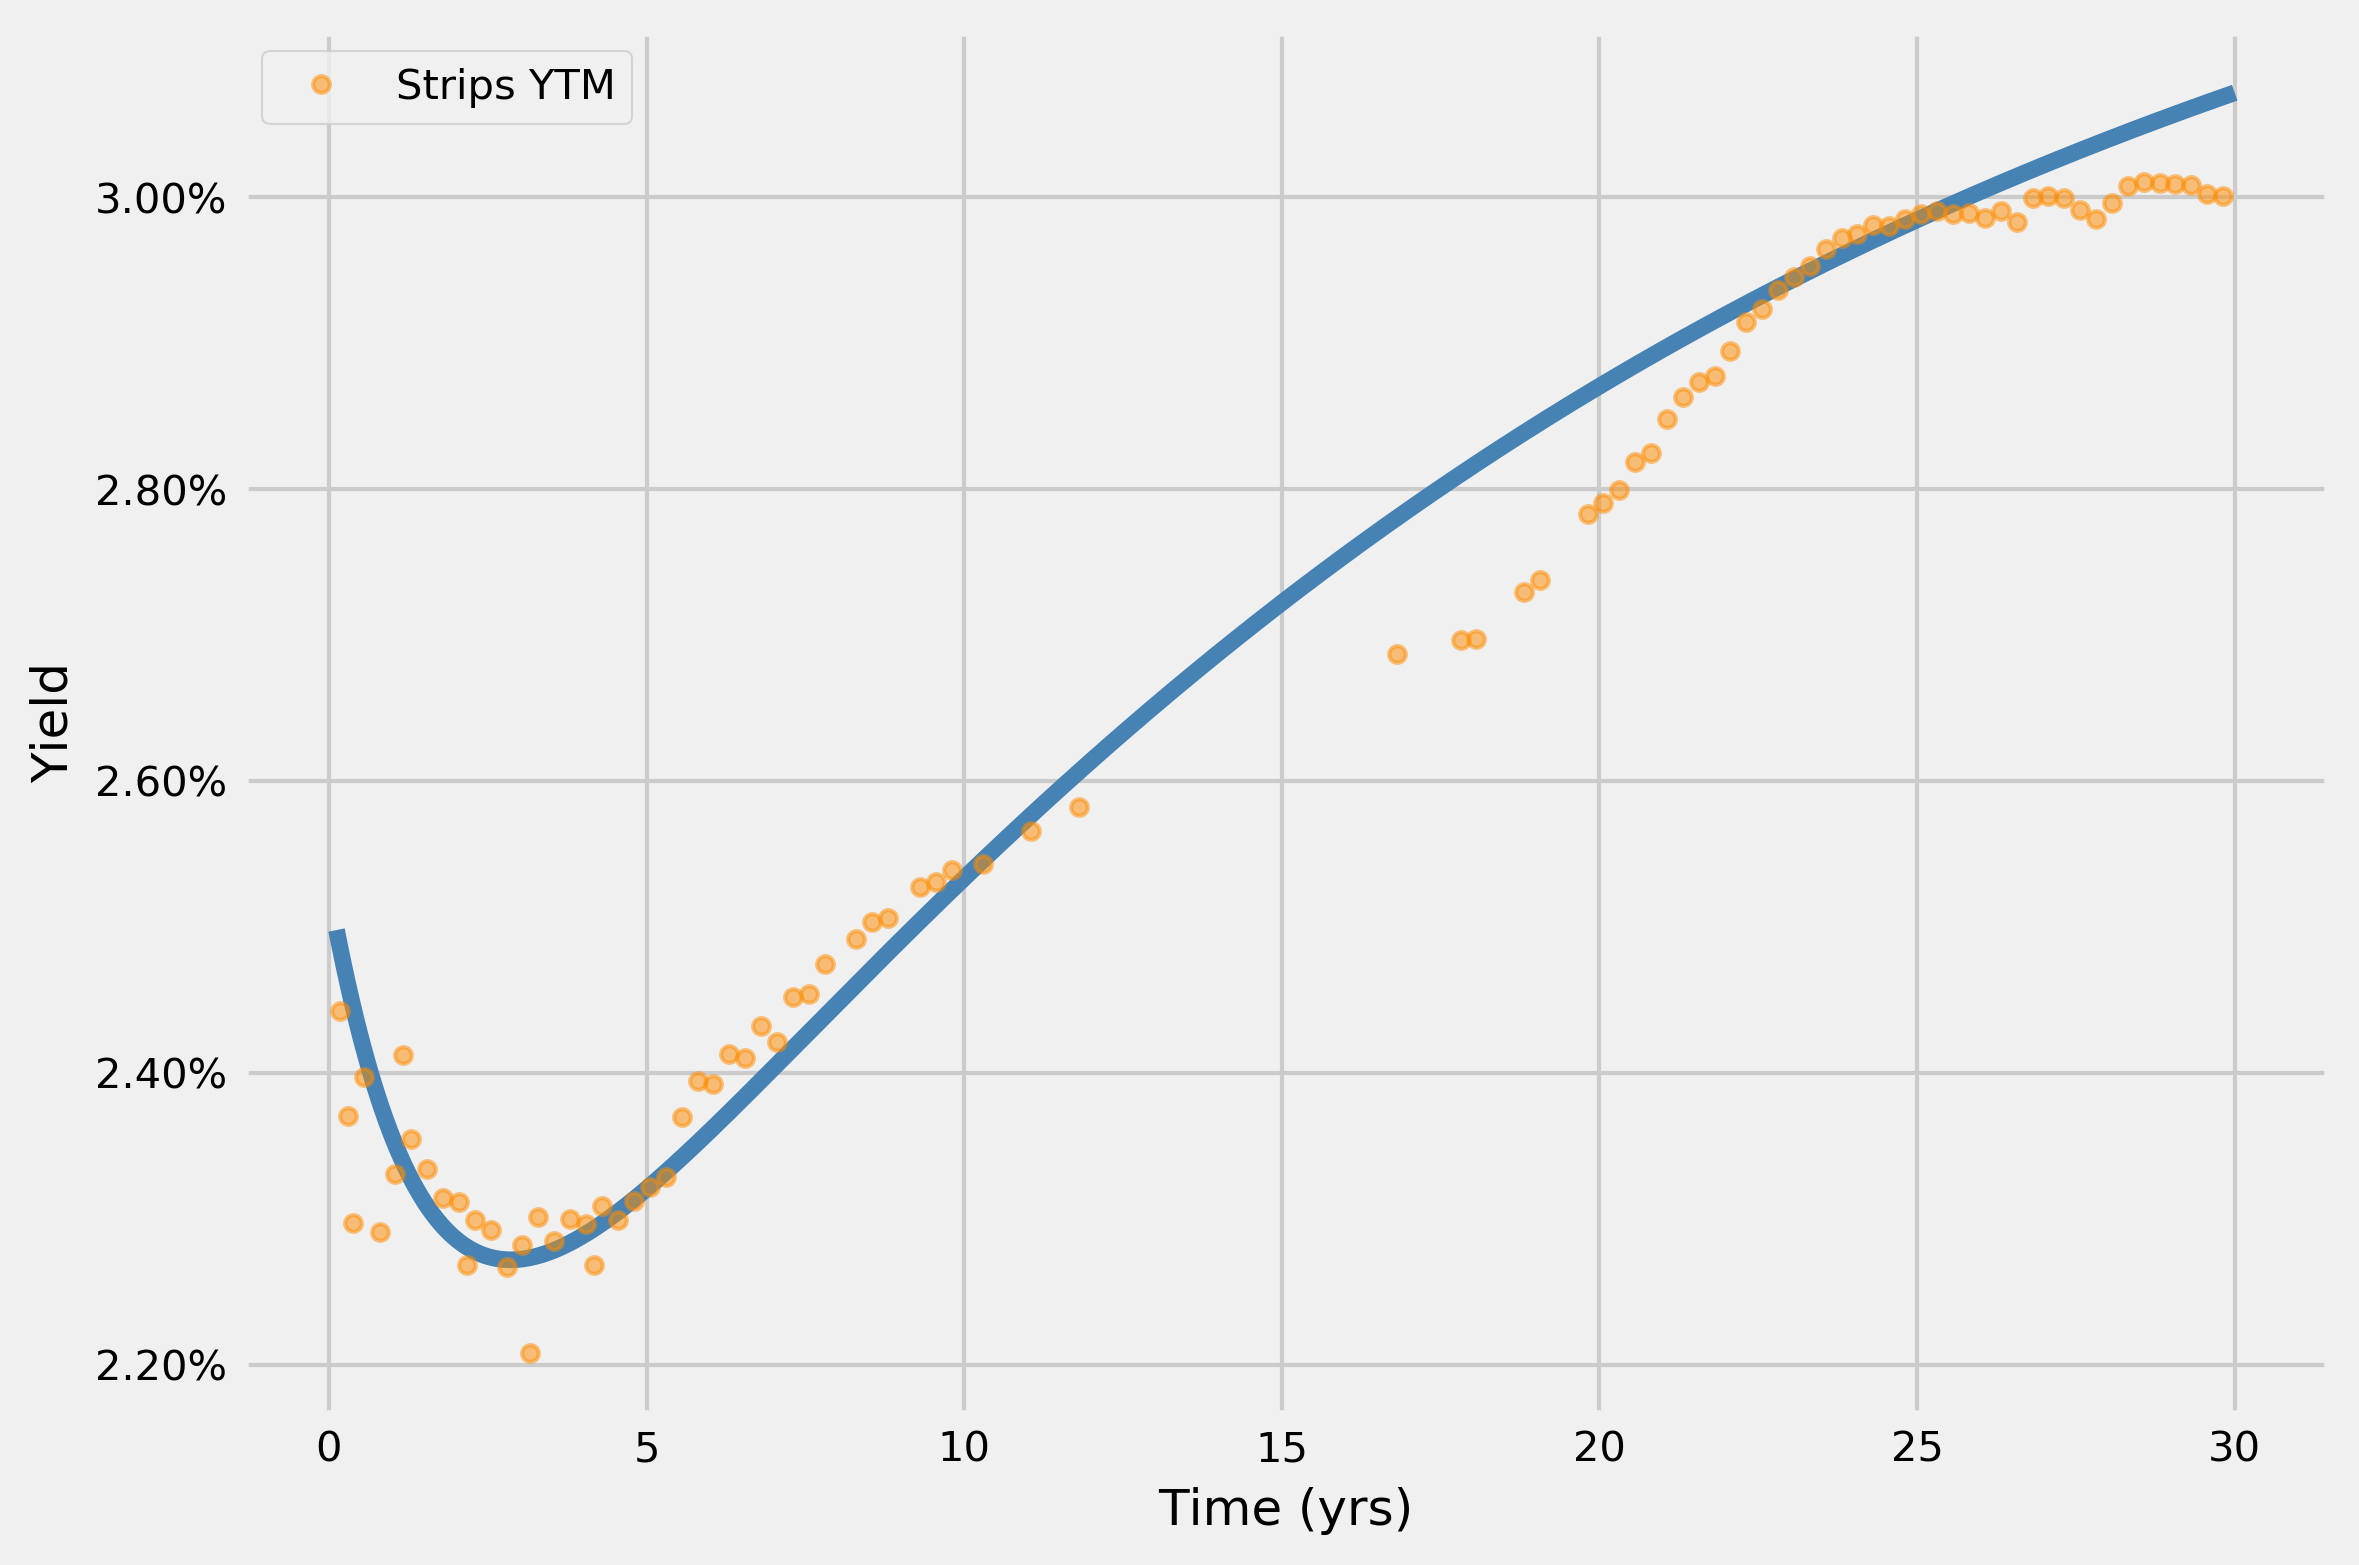
\includegraphics[width=0.9\textwidth]{../../fig/treasury_curves/strips}
	\caption{Zero curve plotted with zero coupon strips' YTMs.}
\end{figure}

For use with key-rate durations, the most important feature of the curve is its consistency. Figure \ref{time} depicts the shifting yield curve over the month of May 2019 in order to show the robust and consistent nature of the curve. During May 2019, the curve had a general parallel shift down with no steepening/flattening or butterflying.

\begin{figure}[H]
	\centering
	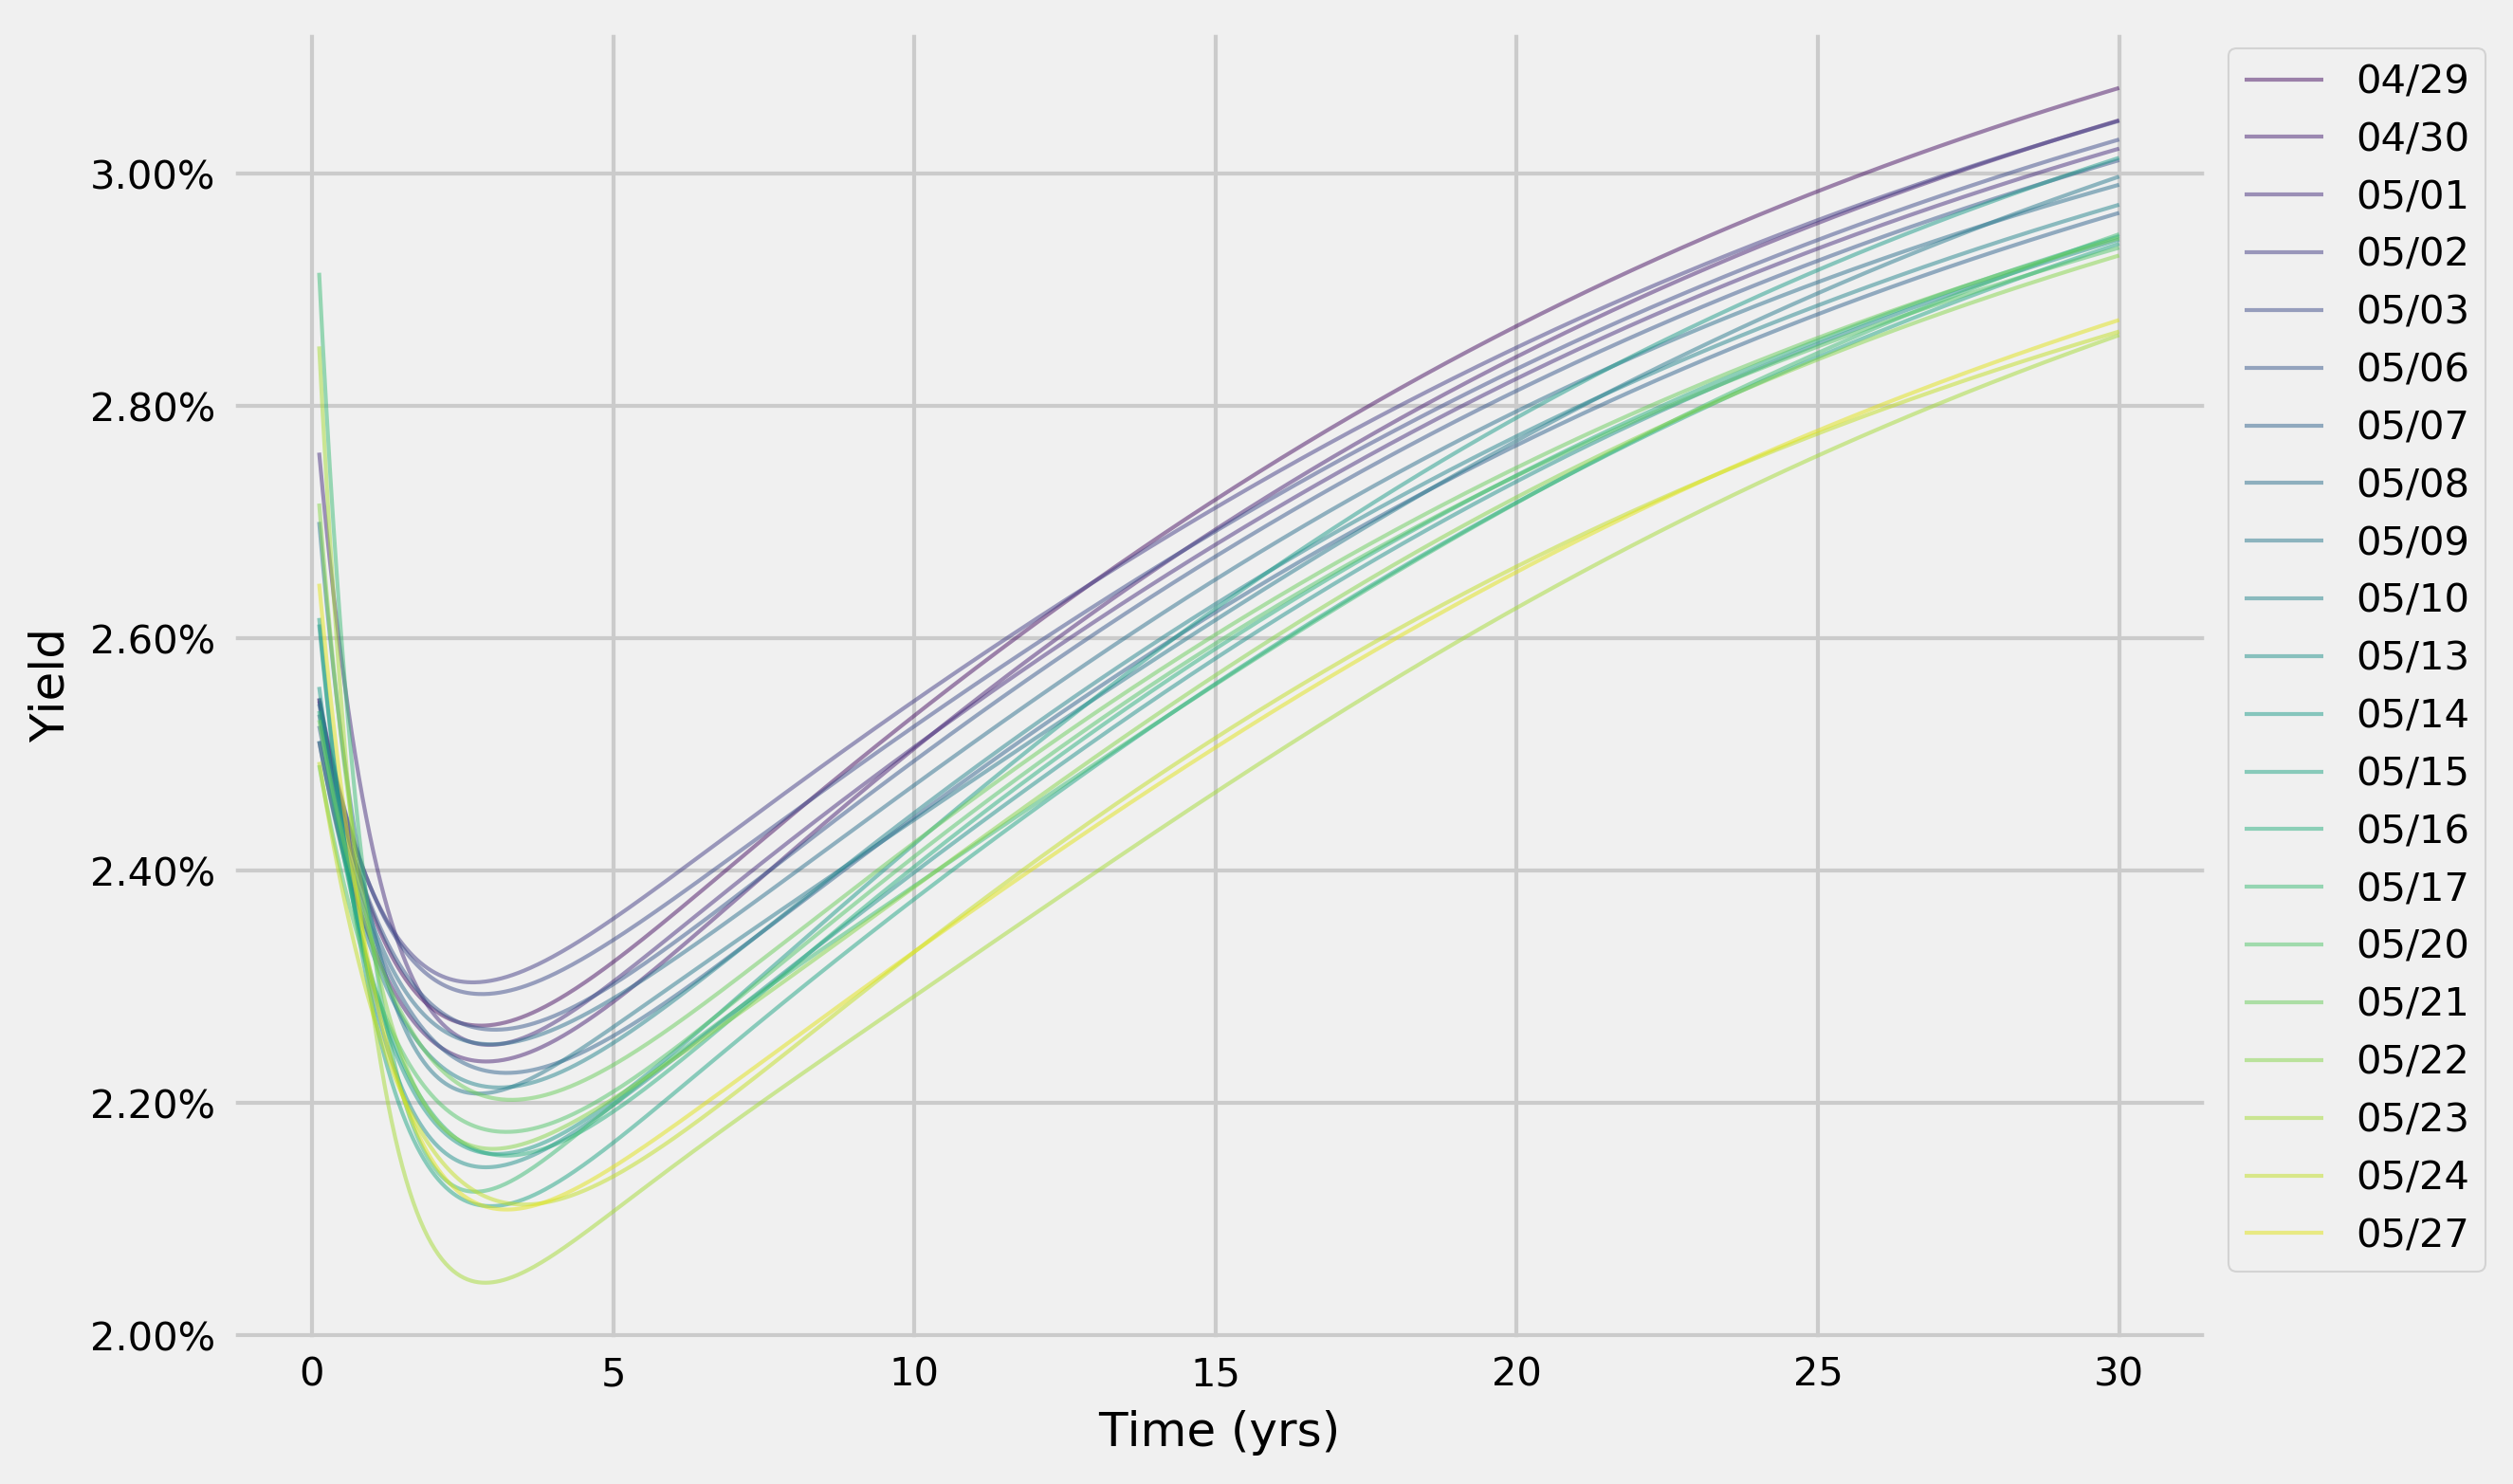
\includegraphics[width=0.9\textwidth]{../../fig/treasury_curves/timeseries}
	\caption{Zero curve plotted over one one month in 2019.}
	\label{time}
\end{figure}

TODO: stress tests. Billy is identifying weeks/months with strange yield curve behavior over the past 20 years to stress test the current algorithm.

\begin{thebibliography}{}
\bibitem{termstrc}
R. Ferstl, \& J. Hayden (2010). 
``Zero-Coupon Yield Curve Estimation with the Package termstrc,'' 
\textit{Journal of Statistical Software}.  \url{http://www.finanzaonline.com/forum/attachments/econometria-e-modelli-di-trading-operativo/1577089d1334234746-diebold-li-improvement-crengi.pdf}

\bibitem{calibrating}
M. Gilli, S. Grobe, \& E. Schumann (2010). 
``Calibrating the Nelson-Siegel-Svensson model,'' 
\textit{Computational Optimization Methods in Statistics, Econometrics, and Finance} 
\url{https://www.jstatsoft.org/article/view/v036i01/v36i01.pdf}
\end{thebibliography}
\end{document}